%%%%%%%%%%%%%%%%%%%%%%%%%%%%%%%%%%%%%%%%%%%%%%%%%%%%%%%%%%%%%%%%%%%%%%%%%%%%%%%%
%%%%%%%%%%%%%%%%%%%%%%%%%%%%%%%%%%%%%%%%%%%%%%%%%%%%%%%%%%%%%%%%%%%%%%%%%%%%%%%%
%%                                                                            %%
%% opintnaytepohja.tex versio 3.01 (2017/10/06)                               %%
%% Opinnäytepohja käytettäväksi aaltothesis.sty (versio 3.01) -tyylitiedoston %%
%% kanssa.                                                                    %%
%% Toimiakseen paketti tarvitsee pdfx.sty v. 1.5.84 (2017/05/18) tai uudempi. %%
%% The LaTeX template file to be used with the aaltothesis.sty (version 3.0)  %%
%% style file.                                                                %%
%% This package requires pdfx.sty v. 1.5.84 (2017/05/18) or newer.            %%
%%                                                                            %%
%% This is licensed under the terms of the MIT license below.                 %%
%%                                                                            %%
%% Copyright 2017, by Luis R.J. Costa, luis.costa@aalto.fi,                   %%
%% Copyright 2017 documentation in Finnish in the template by Perttu Puska,   %%
%% perttu.puska@aalto.fi                                                      %%
%% Copyright Swedish translations 2014 by Elisabeth Nyberg,                   %%
%% elisabeth.nyberg@aalto.fi and Henrik Wallén, henrik.wallen@aalto.fi        %%
%%                                                                            %%
%% Permission is hereby granted, free of charge, to any person obtaining a    %%
%% copy of this software and associated documentation files (the "Software"), %%
%% to deal in the Software without restriction, including without limitation  %%
%% the rights to use, copy, modify, merge, publish, distribute, sublicense,   %%
%% and/or sell copies of the Software, and to permit persons to whom the      %%
%% Software is furnished to do so, subject to the following conditions:       %%
%% The above copyright notice and this permission notice shall be included in %%
%% all copies or substantial portions of the Software.                        %%
%% THE SOFTWARE IS PROVIDED "AS IS", WITHOUT WARRANTY OF ANY KIND, EXPRESS OR %%
%% IMPLIED, INCLUDING BUT NOT LIMITED TO THE WARRANTIES OF MERCHANTABILITY,   %%
%% FITNESS FOR A PARTICULAR PURPOSE AND NONINFRINGEMENT. IN NO EVENT SHALL    %%
%% THE AUTHORS OR COPYRIGHT HOLDERS BE LIABLE FOR ANY CLAIM, DAMAGES OR OTHER %%
%% LIABILITY, WHETHER IN AN ACTION OF CONTRACT, TORT OR OTHERWISE, ARISING    %%
%% FROM, OUT OF OR IN CONNECTION WITH THE SOFTWARE OR THE USE OR OTHER        %%
%% DEALINGS IN THE SOFTWARE.                                                  %%
%%                                                                            %%
%%                                                                            %%
%%%%%%%%%%%%%%%%%%%%%%%%%%%%%%%%%%%%%%%%%%%%%%%%%%%%%%%%%%%%%%%%%%%%%%%%%%%%%%%%
%%                                                                            %%
%%                                                                            %%
%% Esimerkki opinnäytteen tekemisestä LaTeX:lla                               %%
%% Alkuperäinen versio ja kehitystyö Luis Costa, muutokset Perttu Puska       %%
%% Ruotsinkielen tuki lisätty 15092014                                        %%
%% PDF/A-tuki lisätty 15092017                                                %%
%%                                                                            %%
%% Tähän esimerkkiin kuuluu tiedostot                                         %%
%%         opinnaytepohja.tex (versio 3.01)                                   %%
%%         thesistemplate.tex (versio 3.01) (for text in English)             %%
%%         aaltothesis.cls (versio 3.01)                                      %%
%%         kuva1.eps                                                          %%
%%         kuva2.eps                                                          %%
%%         kuva1.pdf                                                          %%
%%         kuva2.pdf                                                          %%
%%                                                                            %%
%%                                                                            %%
%% Kääntäminen Linuxissa joko                                                 %%
%% latex:                                                                     %%
%%             $ latex opinnaytepohja                                         %%
%%             $ latex opinnaytepohja                                         %%
%%                                                                            %%
%%   Tuloksena on tiedosto opinnayte.dvi, joka muutetaan ps-muotoon           %%
%%   seuraavasti                                                              %%
%%                                                                            %%
%%             $ dvips opinnaytepohja -o                                      %%
%%                                                                            %%
%%   ja edelleen pdf-muotoon seuraavasti                                      %%
%%                                                                            %%
%%             $ ps2pdf opinnaytepohja.ps                                     %%
%%                                                                            %%
%% Tai                                                                        %%
%% pdflatex:                                                                  %%
%%             $ pdflatex opinnaytepohja                                      %%
%%             $ pdflatex opinnaytepohja                                      %%
%%                                                                            %%
%%   Tuloksena on tiedosto opinnaytepohja.pdf                                 %%
%%                                                                            %%
%% Selittävät kommentit on tässä esimerkissä varustettu %%-merkeillä ja       %%
%% muutokset, joita käyttäjä voi tehdä, on varustettu %-merkeillä             %%
%%                                                                            %%
%%%%%%%%%%%%%%%%%%%%%%%%%%%%%%%%%%%%%%%%%%%%%%%%%%%%%%%%%%%%%%%%%%%%%%%%%%%%%%%%
%%%%%%%%%%%%%%%%%%%%%%%%%%%%%%%%%%%%%%%%%%%%%%%%%%%%%%%%%%%%%%%%%%%%%%%%%%%%%%%%

%% Käytä yksi näistä:
%% ensimmäinen, jos käytät pdflatexia, joka kääntää tekstin suoraan
%% pdf-tiedostoksi (kuvat on oltava jpg-, png- tai pdf-tiedostoina. Kun teet
%% PDF/A-muotoista pdf-dokumenttia älä käytä PDF/A-muotoista tiedostoa kuvissa.)
%% ja haluat tulostaa opinnäytteesi
%% toinen, jos haluat verkkossa julkaistava PDF/A-muotoista tiedostoa
%% kolmas jos haluat tuottaa ps-tiedostoa (käytä eps-formaattia kuville, älä
%% käytä ps-muotoisia kuvia!)
%%
%\documentclass[finnish, 12pt, a4paper, elec, utf8, pdfa]{aaltothesis}
\documentclass[finnish, 12pt, a4paper, elec, utf8, pdfa, online]{aaltothesis}
%\documentclass[finnish, 12pt, a4paper, dvips]{aaltothesis}

%% Kirjoita y.o. \documentclass optioiksi
%% korkeakoulusi näistä: arts, biz, chem, elec, eng, sci
%% editorisi käyttämä merkkikoodaustapa: utf8, latin1
%% opinnäytetyön kieli: finnish, english, swedish
%% tee arkistointikelpoista PDF/A-1b pdf-tiedosto: pdfa
%% verkkoon menevä symmetrinen taitto ja hypertekstin väri on sininen: online
%%                        (ei optiota on oletusarvo, tuloksena leveä marginaali
%%                         sivun sidonta puolella ja musta hyperteksti)
%% kaksipuolinen tulostus: twoside (oletusarvo on yksipuolinen tulostus)
%%

%% Käytä yksi näistä, jos kirjoitat englanniksi. Katso englanninokset
%% tiedostosta thesistemplate.tex.
%\documentclass[english, 12pt, a4paper, elec, utf8, pdfa]{aaltothesis}
%\documentclass[english, 12pt, a4paper, elec, utf8, pdfa, online]{aaltothesis}
%\documentclass[english,12pt, a4paper, dvips]{aaltothesis}

\usepackage{graphicx}

%% Matematiikan fontteja, symboleja ja muotoiluja lisää, näitä tarvitaan usein
\usepackage{amsfonts,amssymb,amsbsy}


%% Korjaa vastaamaan korkeakouluasi, jos automaattisesti asetettu nimi on
%% virheellinen
%%
%% Change the school field to specify your school if the automatically
%% set name is wrong
% \university{aalto-yliopisto}
% \school{Sähkötekniikan korkeakoulu}

%% Korjaa seuraava vastaamaan koulutusohjelmaasi
%%
\degreeprogram{Sähkötekniikan kandidaattiohjelma}
%%

%% Pääaineesi
\major{Automaatio ja systeemitekniikka}

%% Pääainekoodi
%%
%%\code{}
%%

%% Valitse yksi näistä kolmesta
%%
\univdegree{BSc}
%\univdegree{MSc}
%\univdegree{Lic}
%%

%% Oma nimi
%%
\thesisauthor{Joni Airaksinen}
%%

%% Opinnäytteen otsikko tulee tähän ja mahdollisesti uudelleen englannin- tai
%% ruostinkielisen abstraktin yhteydessä. Älä tavuta otsikkoa ja vältä liian
%% pitkää otsikkotekstiä. Jos latex ryhmittelee otsikon huonosti, voit joutua
%% pakottamaan rivinvaihdon \\ kontrollimerkillä.
%% Tällöin...
%% Muista että otsikkoja ei tavuteta!
%% Jos otsikossa on ja-sana, se ei jää rivin viimeiseksi sanaksi vaan aloittaa
%% uuden rivin.
%% Anna ostikko uudelleen ilman rivinvaihtomerkkiä optionaalisena argumenttina
%% hakasuluissa. Näin tehdään, koska otsikko on osaa pdf/a-tiedostossa olevaa
%% metadataa, ja metadatassa ei saa olla rivinvaihtomerkkiä.
%%
\thesistitle{KANDIDAATINTYÖ}
%\thesistitle[Opinnäytteen otsikko]{Opinnäyteen\\ otsikko}
%%

\place{Espoo}

%% Kandidaatintyön päivämäärä on sen esityspäivämäärä!
%%
\date{23.4.2018}
%%

%% Kandidaattiseminaarin vastuuopettaja tai diplomityön valvoja.
%% Huomaa tittelissä "\" -merkki pisteen jälkeen, ennen välilyöntiä ja
%% seuraavaa merkkijonoa.
%% Näin tehdään, koska kyseessä ei ole lauseen loppu, jonka jälkeen tulee
%% hieman pidempi väli vaan halutaan tavallinen väli.
%%
\supervisor{TkT.\ Pekka Forsman}
%%

%% Kandidaatintyön ohjaaja(t) tai diplomityön ohjaaja(t). Ohjaajia saa
%% olla korkeintaan kaksi.
%%
%\advisor{Prof.\ Pirjo Professori}
\advisor{TkL Pekka Aarnio}
%\advisor{DI Tina Tutkija}
%%

%% Aaltologo: syntaksi:
%% \uselogo{aaltoRed|aaltoBlue|aaltoYellow|aaltoGray|aaltoGrayScale}{?|!|''}
%% Logon kieli on sama kuin dokumentin kieli
%%
\uselogo{aaltoRed}{''}
%%

%% Suomenkielinen tiivistelmä:
%% Kaikki tiivistelmässä tarvittava tieto (nimesi, työnnimi, jne.) käytetään
%% niin kuin se on yllä määritelty.
%% Tiivistelmän avainsanat:
%% Huom! Avainsanat erotetaan toisistaan \spc -makrolla
%%
\keywords{Semanttinen verkko\spc RDF\spc}

%% Tiivistelmän tekstiosa. Tämä teksti sisältyy pdf-tiedoston metadataa ja tulee
%% myös tiivistelmälomakkeeseen.
%%
\thesisabstract{
Tiivistelmässä on lyhyt selvitys (noin 100 sanaa) kirjoituksen tärkeimmästä
sisällöstä: mitä ja miten on tutkittu, sekä mitä tuloksia on saatu. Tämän
opinnäytteen Pdf/A -formaatissa tiivistelmäteksti kirjoitetaan opinnäytteen
luettavan osan lomakkeen lisäksi myös pdf-tiedoston metadataan. Kirjoita tähän
metadataan kirjoitettavaa teksti. Metadatatekstissa ei saa olla erikoismerkkejä,
rivinvaiho- tai kappaleenjakomerkkiä, joten näitä merkkeja ei saa käyttää tässä.
Jos tiivistelmäsi ei sisällä erikoimerkkejä eikä kaipaa kappaleenjakoa, voit
hyödynttää makroa abstracttext luodessasi lomakkeen tiivistelmää (katso
kommentti alla). Metadatatiivistelmatekstin on muuten oltava sama kuin
lomakkeessa oleva teksti.
}

%% Tekijänoikeusteksti. Tekijänoikeus on tekijällä riippumatta siitä onko
%% copyright -merkintä näkyvissä vai ei. Halutessasi voit jakaa työsi Creative
%% Commons -lisensillä (katso creativecommons.org), jolloin lisenssitekstin on
%% oltava näkyvissä. Kirjoita tähän haluamasi tekijänoikeustekstin. Se kirjautuu
%% myös pdf-tiedoston metadataan.
%% Syntaksi:
%% \copyrigthtext{metadatateksti}{sivulle näkyviin tuleva teksti}
%%
%% A.o. metadataan menevässä tekstissä on käytettävä \noexpand -makroa ennen
%% \copyright -erikoismerkkiä ja makrot (tässä \copyright ja \year) on erotettava
%% seuraavasta tekstistä \ -merkillä (välilyöntimerkki). \copyrighttext-makron
%% argumentissa olevat makrot automaattisesti hakevat vuosiluvun ja tekijän nimi.
%% (Huom! \ThesisAuthor on aaltothesis.cls -tyylitiedoston sisäinen makro).
%% Toki saman tekstin olisi voinut kirjoittaa yksinkertaisesti näin:
%% \copyrighttext{Copyright \noexpand\copyright\ 2017 Teemu Teekkari}
%% {Copyright \copyright{} 2017 Teemu Teekkari}
%%
\copyrighttext{Copyright \noexpand\copyright\ \number\year\ \ThesisAuthor}
{Copyright \copyright{} \number\year{} \ThesisAuthor}

%% Voit estää LaTeXia kirjoittamasta xmpdata-tiedostoon (sisältää pdf-tiedostoon
%% kirjoitettavaa metadataa) asettamalla writexmpdatafile lipun arvoksi 'false'.
%% Tämä mahdollistaa sen, että voit kirjoittaa metadataa suoraan oikeassa
%% muodossa tiedostoon opinnaytepohja.xmpdata.
%%
%\setboolean{writexmpdatafile}{false}

%%-------------------------------------------------------------------------------
%% OMAT ASETUKSET:
%% Aseta tyjä rivi kappaleiden väliin
\usepackage[parfill]{parskip}

%% Vaihdetaan sisällysluettelon väri mustaksi
\usepackage{hyperref}% http://ctan.org/pkg/hyperref
\hypersetup{%
  colorlinks = true,
  linkcolor  = black
}

%% Seuraavalla päästään eroon turhista \hbox warningeista:
\usepackage{etoolbox}
\apptocmd{\sloppy}{\hbadness 10000\relax}{}{}

\usepackage{listings}

%% Salli svg kuvat
\usepackage{svg}
\usepackage{amsmath}
%%-------------------------------------------------------------------------------


%% Kirjoitelman alku
\begin{document}

%% Tehdään kansilehti
%%
\makecoverpage

%% Tehdään tekijänoikeusteksti näkyväksi.
%% Halutessasi voit jättää tekijänoikeustekstin pois luettavasta pdf-tiedostosta.
%% Tämä voi tuntua hyvältä ajatukselta paperille tulostetulla versiossa eteenkin,
%% jos sivun ainoa teksti on "Copyright (c) vvvv Teemu Teekkari". Suositus on
%% kuitenkin jättää teksti näkyviin.
%%
\makecopyrightpage

%% Suomenkielinen tiivistelmä
%% Kaikki tiivistelmässä tarvittava tieto (nimesi, työnnimi, jne.) käytetään
%% niin kuin se on yllä määritelty.
%%
%% Tiivistelmän tekstiosa
%%
\begin{abstractpage}[finnish]
Tiivistelmässä on lyhyt selvitys (noin 100 sanaa) kirjoituksen tärkeimmästä
sisällöstä: mitä ja miten on tutkittu, sekä mitä tuloksia on saatu.

Tämän opinnäytteen Pdf/A -formaatissa tiivistelmäteksti kirjoitetaan
opinnäytteen luettavan osan lomakkeen lisäksi myös pdf-tiedoston metadataan
$\backslash$thesisabstract-makron avulla (kasto yllä). Kirjoita tähän
luettavaan tiivistelmälomakkeeseen menevä teksti. Tässä saa olla erikoismerkkejä
kuten kreikkalaiset kirjaimet ja rivinvaiho- ja kappaleenjakomerkit. Tämän
tekstin on muuten oltava sama kuin metedatatiivistelmän teksti.

Jos tiivistelmäsi ei sisällä erikoimerkkejä eikä kaipaa kappaleenjakoa, voit
hyödynttää makroa $\backslash$abstracttext luodessasi lomakkeen tiivistelmää
(katso kommentti alla).
\end{abstractpage}

%% \thesisabstract -makrossa kirjoitettu teksti on tallennettu \abstractext
%% -makrosa jolloin voit siirtää metadataan menevä teksti sellaisenaan näin:
%%
%\begin{abstractpage}[finnish]
%	\abstracttext{}
%\end{abstractpage}

%% Pakotetaan uusi sivu varmuuden vuoksi, jotta mahdollinen suomenkielinen ja
%% englanninkielinen tiivistelmä eivät tule vahingossakaan samalle sivulle
%%
\newpage





%% Esipuhe
%%
\mysection{Esipuhe}
tmp

\vspace{5cm}
Otaniemi, 15.9.2017

\vspace{5mm}
{\hfill Joni Airaksinen \hspace{1cm}}

%% Pakotetaan varmuuden vuoksi esipuheen jälkeinen osa
%% alkamaan uudelta sivulta
\newpage


%% Sisällysluettelo
%%
\thesistableofcontents


%% Symbolit ja lyhenteet
%%
\mysection{Symbolit ja lyhenteet}

\subsection*{Symbolit}

\begin{tabular}{ll}
%%$\mathbf{B}$  & magneettivuon tiheys  \\
\end{tabular}

\subsection*{Operaattorit}

\begin{tabular}{ll}
%$\nabla \times \mathbf{A}$              & vektorin $\mathbf{A}$ roottori\\
\end{tabular}

\subsection*{Lyhenteet}
\begin{tabular}{ll}
OWL          & Web Ontology Language \\
RDF          & Resource Description Framework \\
SPARQL       & SPARQL Protocol and RDF Query Language \\
WWW          & World Wide Web \\
W3C          & World Wide Web Consortium \\
XML          & Extensible Markup Language \\
\end{tabular}


%% \clearpage on melkein samanlainen kuin newpage, mutta
%% flushaa myös LaTeX:n floatit
%%
\cleardoublepage

%% MEMO:
%% Tietämyksen esittämiskieli
%%
%%
%% Selitä metadata?
%%
%% Internet sana isolla, koska se korostaa sanaa. Internet sana on lauseissa
%% yleensä hyvin merkityksellinen, joten on hyvä jos se erottuu muiden seasta.
%%
%% "This classical layer cake was a major driver in the agenda of the Semantic Web,
%%ut is now quite outdated" (PRIMER, s.18) - älä esittele kakkumallia?

%%===============================================================================
%% Leipäteksti alkaa
\section{Johdanto}

%% Ensimmäinen sivu tyhjäksi
\thispagestyle{empty}
Internet mahdollistaa suurten tietomäärien jakamisen. Nykyisin informaatiota on kuitenkin niin paljon tarjolla, että yksittäinen ihminen ei kykene käymään kaikkea tietoa lävitse, joten merkityksellistä informaatiota täytyy pystyä valikoimaan. Semanttinen verkko tietotekniikan tutkimusalana pyrkii vastaamaan tiedon valikointiongelmaan standardoimalla menetelmiä joiden avulla tietokoneet pystyvät jäsentämään tietoa.

Tietokoneiden ymmärtämä jäsennelty tieto on erittäin arvokasta. Tietokoneet voivat jalostaa jäsenneltyä tietoa itsenäisesti pidemmälle, jolloin ne kykenevät löytämään uusia asiayhteyksiä. Asiayhteydet voivat olla täysin tuntemattomia ihmiselle, jolloin niiden esittämisestä voi olla hyötyä käyttäjälle. Semanttisen verkon tarkoituksena on siis tehdä Internetistä ja tietokoneista entistäkin hyödyllisempiä, koska tietokoneiden resurssit riittävät nykyisin muuhunkin kuin pelkästään tiedon esittämiseen ja jakamiseen. Tietokoneiden ei tarvitse olla ainoastaan ihmisen työkaluja vaan ne voivat olla myös apureita.

Tietokoneet eivät ymmärrä tiedon välisiä suhteita suoraan tekstistä kuten ihmiset. Sanat ja lauseet itsessään eivät tarkoita tietokoneelle mitään. Sanat koostuvat erilaisista kirjainyhdistelmistä, jotka voidaan esittää binääreinä \cite{ASCII}, mutta näiden avulla ei voida luoda asiayhteyksiä. Tietokone ei esimerkiksi kykene tunnistamaan synonyymejä terveyskeskus ja terveysasema, vaan tietokone käsittää ne täysin erillisinä sanoina. Tästä syystä tarvitaan lisätietoa, jonka avulla tietokoneelle voidaan kertoa sanojen merkitys ja suhde. Suhteiden kuvaamista varten on kehitetty tietämyksenesittämiskieliä. Yksi onnistunut ja hyvin spesifioitu tietämyksenesttämiskieli on Web Ontology Language (OWL) \cite{OWL_specification}. Jotta OWL:lla kyketään kuvaamaan suhteita, niin tarvitaan standardoitu tietomalli. Semanttisen verkon yhteydessä tietomalli on lähes poikkeuksetta RDF (Resource Description Framework), joka on W3C:n spesifioima \cite{RDF_specification} tietomalli. Tietomallilla voidaan kuitenkin ainoastaan säilöä tietoa sopivassa muodossa, joten tarvitaan vielä menetelmiä säilötyn tiedon hakemiseen. RDF tiedon hakemiseen käytetään SPARQL (SPARQL Protocol and RDF Query Language) kyselykieltä.

Tutkielmassa tullaan käymään edellämainitut semanttisen Internetin peruselementit yksitellen lävitse. Tarkoituksena on muodostaa kuva siitä, mitä menetelmiä semanttisen Internetin toteutuksessa vaaditaan. Samoin tutkielma pyrkii selventämään semanttisen Internetin käsitettä lukijalle, koska kovinkaan moni ei tunne termin merkitystä, vaikka hyödyntää semanttisia verkkoja päivittäin. Tutkielmassa tullaan siis ensimmäiseksi käsittelemään semanttista Internetiä kokonaisuudessaan. Toisessa luvussa syvennytään toteutukseen. Kolmannessa luvussa pohditaan tiedon suhteisuutta ja tämän merkitystä tietokoneiden kontekstissa. Neljännessä luvussa tuodaan ilmi semanttisen Internetin edistys ja pyritään luomaan järkevä ennuste tulevaisuudesta. Lopuksi asiat kiteytetään yhteen.


\clearpage %% Opinnäytteessä jokainen osa alkaa uudelta sivulta, joten \clearpage
%%===============================================================================
\section{Semanttinen verkko kokonaisuutena}


Semanttinen verkko ei pyri vastaamaan mihinkään yksittäiseen ongelmaan, vaan se mahdollistaa uusien asioiden toteuttamisen ja tiedon tehokkaamman hyödyntämisen.
Vuonna 2001 Bernenrs-Lee ja hänen kollegansa esittelevät, että ei ole mitään yksittäistä sovellusta, minkä vuoksi Internet on äärimmäisen menestynyt. He totesivat, että semanttinen verkko tulee olemaan vastaavanlainen ilmiö, joka tulee mahdollistamaan uusia ennenäkemättömiä asioita \cite{Berners_visio}. Tuolloin Berners-Leen puheet saattoivat kuulostaa utopistisilta, koska mitään konkreettista havainnoinnnkohdetta ei ollut tarjota ja kukaan ei osannut suoraan sanoa mihin semanttista Internetiä tulee käyttää. Onneksi asiaa on kuitenkin helpompi ymmärtää nykyään, koska meidän ympäriltä löytyy useita sovelluksenkohteita, jotka hyödyntävät semanttista Internetiä. Esimerkiksi Facebook käyttää semanttista verkkoa tiedonhaussa, jolloin se kykenee tarjoamaan käyttäjälle parempia hakutuloksia \cite{Facebook}.


Semanttinen Internet ei synny itsestään vaan vaatii ihmisen tekemää työtä. Tietokoneet eivät kykene havaitsemaan suhteita tekstin ja sanojen välillä, vaan suhteet täytyy kertoa niille erikseen. Asioiden suhteita pystytään ilmoittamaan monella erilaisella tavalla, mutta on hyödyllistä mikäli kaikki pyrkivät yhtenäiseen merkintätapaan. Tämä mahdollistaa sen, että eri sovellukset voivat kommunikoida keskenään ilman ylimääräistä vaivannäköä. Näin tiedon jakaminen saadaan mahdollisimman tehokkaaksi. Antonious et.al tiivistää semanttisen verkon menetelmien suunnitteluperiaatten kolmeessa pääkodassa. Ensinnäkin Internetissä olevan informaation tulisi olla saatavilla standardoidussa muodossa. Tietoelementtien ja niiden keskenäisten suhteiden tulisi olla tietokoneiden saatavissa sen sijaan, että esitettäisiin ainoastaan tietoa itsessään. Kolmantena periaatteena on esittää tiedon keskenäiset suhteet sellaisessa muodossa, että tietokoneet voivat käsitellä suhteita \cite{Antoniou}. Kun edellämainitut periaatteet täyttyvät, niin Internetissä olevan tiedon hyödyntäminen ei rajoitu ainoastaan ihmiseen.

World Wide Web Consortium (W3C) on ottanut tehtäväkseen kehittää yhteisiä Internetiin liittyviä standardeja. Tästä syystä W3C onkin vastuussa useista semanttisen verkon standardeista, jotka pyrkivät noudattamaan edellämainittuja suunnitteluperiaatteita. Samoin termi semanttinen Internet on peräisin Berners-Leeltä, joka on Internetin kehittäjä ja W3C:n johtajan. \cite{W3C}. Berners-Lee esittelee semanttisen webin Internetin jatkeena, joka mahdollistaa ihmisten ja tietokoneiden yhteistyön \cite{Berners_visio}.





Vuonna 2001 Berners Lee visioi konfiguroinnin helpottuvan, kun laitteita kyetään ohjaamaan niistä saatavan semanttisen tiedon avulla. Hän aluksi kuvailee kuinka kotiautomaation konfigurointi vaatii useiden laitteiden huolellista konfigurointia, mutta semantiikan avulla voisi riittää, että ohjelmointi/konfigurointi tehtäisiin ainoastaan kerran \cite{Berners_visio}.







\clearpage
%%===============================================================================
\section{Semanttisen verkon peruskomponentit}

\subsection{XML}
XML (eXtensible Markup Language) on W3C:n standardoima merkintäkieli, jonka avulla voidaan tallentaa ja siirtää tietoa. XML on suunniteltu niin, että sitä voi lukea sekä ihminen että tietokone. Merkinnältään XML muistuttaa hyvin paljon HTML merkintäkieltä, mutta XML:n keskeisimpänä erona on toimia mielivaltaisen tiedon tallennuskielenä, kun taas HTML:llä pystytään esittämään ainoastaan ennalta määriteltyjä rakenteita \cite{IEEE_XML}. XML:n joustavuus mahdollistaa sen, että kaikenmuotoinen tieto voidaan tallentaa yksittäisessä standardi muodossa. Tämän ansiosta erilaiset tietomuodot eivät aiheuta rajoitteita. Riittää, että semanttinen sovelluksemme osaa lukea yhtä kieltä kymmenen sijaan. Edellinen ajatus kuitenkin vaatii sen, että joku tai jokin serialisoi eli kääntää alkuperäisen tiedon XML muotoon.

Esimerkki XML-syntaksista:
%%\lstinputlisting[language=Xml]{production_file.xml}
%% name voisi olla myös product attribuutti
\begin{lstlisting}
<sweet_roast>
  <product>
    <name>Herkkupaahto</name>
  </product>
</sweet_roast>
\end{lstlisting}

XML ei yksinään riitä semanttisen tiedon esittämiseen, koska merkinnästä nähdään ainoastaan tiedon rakenne. Rakenteen esittämisen lisäksi meidän tulisi myös pystyä yhdistämään tiedonpalasia toisiinsa. Tästä syystä XML syntaksia täytyy laajentaa tai vaihtoehtoisesti meidän tulee käyttää muita menetelmiä.

%% METADATA?
%% TIETOA DATASTA.

\subsection{RDF(S)}
%%s.18 primer
RDF on semanttisen internetin tietomalli.

RDF:n erikoisuus on sen joustavuus. RDF on suunniteltu niin, että sillä pystytään kuvaamaan kaikenlaista tietoa internetissä, jolloin se soveltuu kaikkialle \cite{RDF_specification}.

RDF tieto koostuu kolmikoista (engl. triple).


RDF:n joustavuutta ei kuitenkaan saavuteta ilmaiseksi. Tietokoneen tulee osata yhdistää samankaltaista, mutta eri sivustoilla esitettyä tietoa. Samasta asiasta saatetaan puhua eri nimityksillä eri sivustoilla. Tästä syystä ..., joka tehdään RDFS:n avulla (Resource Description Framework Schema)

Hyvin usein termillä "RDF" viitataan sekä RDF:ään että RDFS:ään.

\subsubsection{Kolmikko}
%% Lukijan odotetaan tietävän mitä tarkoittaa URL ja ISBN
RDF esitys vaatii, että kaikki resurssit esitetään uniikeilla tunnisteilla. Uniikkia tunnistetta nimitetään URI:ksi (URI – Unique Resource Identifier) ja tunniste voi esimerkiksi olla URL (Uniform Resource Locator), ISBN tai vaikkapa puhelinnumero. URI:n avulla tietokone kykenee ymmärtämään yksiselitteisesti mihin viitataan.

RDF tietomallissa kuvataan resurssien välisiä suhteita. Resurssien välisiä suhteita kutsutaan predikaateiksi tai vaihtoehtoisesti ominaisuuksiksi. Esimerkiksi ominaisuudella "omistaa" voidaan kuvata kuinka asia A omistaa asian B. Asiasuhteiden hahmottaminen on ihmiselle melko autonomista, mutta tietokoneet eivät lähtökohtaisesti kykene muodostamaan suhteita itsenäisesti. Siksi suhteet täytyy kertoa erikseen, jotta tietokone voi havaita kahden asian välillä vallitsevan merkityksen.


Kolmantena tärkeänä RDF:n ominaispiirteenä esiintyy toteamukset (engl. statements). Toteamukset yhdistävät edelläesitellyt resurssit ja predikaatit yhdeksi kokonaisuudeksi. Toteamus koostuu resurssista, ominaisuudesta ja määrätystä arvosta. Arvo voi olla esimerkiksi jokin numero, merkkijono, päivämäärä tai toinen resurssi. Voidaan siis sanoa, että toteamukset koostuvat aina subjektista, predikaatista ja objektista. Tästä syystä sanotaan, että RDF tietomuodossa oleva tieto koostuu kolmikoista (engl. triple).


Kolmikot voidaan esittää graafimaisessa muodossa Kuva 1:n tapaan. Kaaviot saattavat auttaa kokonaisuuden hahmottamisessa, jonka vuoksi niitä käytetään havainnollistamisen tukena. Tulee kuitenkin huomata, että mitään yksittäistä standardia ei ole olemassa RDF-graafeille, minkä vuoksi seuraavat kaaviot ovat vain yksi mahdollinen esitysmuoto monien joukosta. On myös hyvä tiedostaa, että jokaiseen resurssiin viitataan todellisuudessa URI:n avulla, mutta kaaviossa URI:t on jätetty selvyyden vuoksi pois.

%% Graafi
\begin{figure}[htb]
\centering
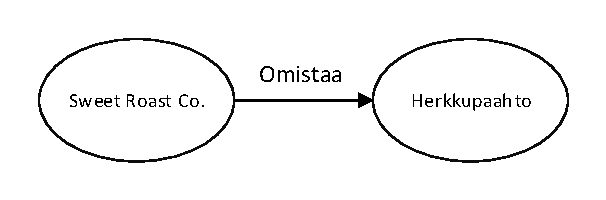
\includegraphics[height=3cm]{images/RDF-triplet1.pdf}
\caption{Esimerkki graafi tripletistä. \label{images/RDF-triplet1}}
\end{figure}


\subsubsection{XML/RDF}
Kaavion kahviyhtiö "Sweet Roast Co." on subjektin asemassa. Yhtiö omistaa kahvituotteen Herkkupaahto. "Omistaa" on siis predikaatti ja "Herkkupaahto" on objekti. Yhdessä nämä muodostavat kolmikon, josta on mahdollista havaita rakenne sekä kahvintuotteen ja yhtiön välinen suhde. Tietokoneet eivät kuitenkaan osaa lukea kaaviota, joten tieto täytyy pystyä esittämään jollain toisella tavalla. Standardoitu RDF/XML tietomalli mahdollistaa tiedon esittämisen tietokoneelle ymmärrettävässä muodossa. Syntaksi on hiukan tavallista XML:ää laajempi, jolloin myös suhteet pystytään esittämään.

%% XML/RDF example
%% hasProduct instead of product
\vskip 0.75cm
\begin{lstlisting}
<rdf:RDF
xmlns:rdf="http://www.w3.org/1999/02/22-rdf-syntax-ns#"
xmlns:sr="http://www.SweetRoast.com/semantics/relationship#">

<rdf:Description
rdf:about="http://www.SweetRoast.com">
  <sr:product rdf:resource="http://www.SweetRoast.com/product/herkkupaahto"/>
</rdf:Description>
</rdf:RDF>
\end{lstlisting}
\vskip 0.75cm


\begin{figure}[htb]
\centering
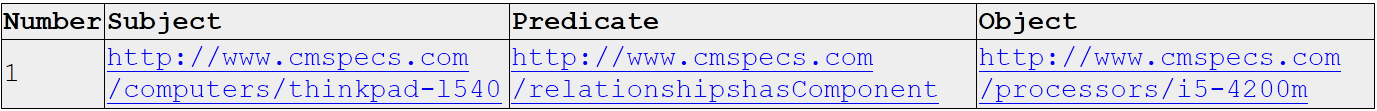
\includegraphics[width=15cm]{images/RDF-valid.PNG}
\caption{Suhteet talukoituna. Lähde: \cite{W3C_RDF_validator}. \label{images/RDF-triplet1}}
\end{figure}
\cite{W3C_RDF_validator}.

Ylläoleva kuva on generoitu automaattisesti XML/RDF merkinnän pohjalta käyttäen W3C:n palvelua. Voimmekin havaita, että ulkopuolinen palvelu on ymmärtänyt esimerkkimme rakenteen oikein. Palvelu on löytänyt subjektiksi kahviyhtiömme, objektiksi kahvituotteemme ja predikaatiksi oikean suhteen. Suhteen tulisi siis olla erikseen määriteltynä osoitteessa: \url{http://www.SweetRoast.com/semantics/relationship\#product}. Tietokoneet kykenevät siis nyt havaitsemaan yhteyden kahvituotteen ja kahviyhtiön välillä, kun ne hyödyntävät semsanttisen internetin menetelmiä.

\subsubsection{Turtle}
Nykyisin RDF:ää kirjoitettaessa suositaan kuitenkni paljon muitakin syntakseja kuin pelkkää XML:ää. Esimerkiksi Turtle (Terse RDF Triple Language) on tällähetkellä hyvin suosittu syntaksi sen helpon luettavuuden ja kirjoitettavuuden vuoksi. Turtle mukailee laajempaa Notation 3 (N3) syntaksia. Seuraavassa on kahviesimerkin rakenne kirjoitettu Turtlella:

%%Turle example
\vskip 0.75cm
\begin{lstlisting}
@prefix rdf: <http://www.w3.org/1999/02/22-rdf-syntax-ns#> .
@prefix sr: <http://www.SweetRoast.com/semantics/relationship> .

<http://www.SweetRoast.com/>
  sr:product <http://www.SweetRoast.com/product/herkkupaahto/> .
\end{lstlisting}
\vskip 0.75cm


\begin{figure}[htb]
\centering
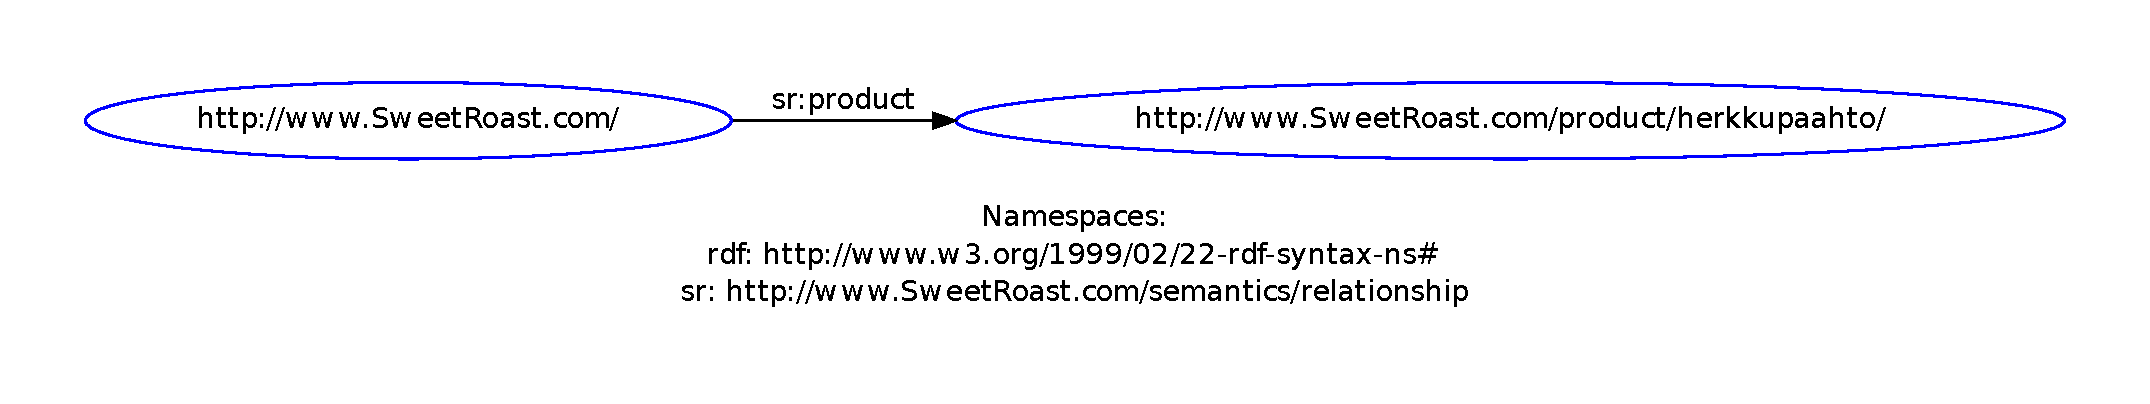
\includegraphics[width=15cm]{images/RDF-triplet2.pdf}
\caption{Turtle syntaksista automaattisesti generoitu graafi. Lähde: \cite{SeCo_RDF_validator} \label{images/RDF-triplet2}}
\end{figure}


%%:atomicNumber 2 ;
Esimerkeistä olisi hyvä huomata, että tietorakenteet eivät ole täysin identtisiä, mutta hyvin lähellä toisiaan. Tämä johtuu merkintäkielien avoimesta luonteesta, jonka ansiosta merkintäkielet sopivat kaikkialla käytettäväksi. Tärkein ominaisuus on se, että tietoa ei katoa mihinkään. Päinvastoin, Tietoa tulee lisää, kun tarkennamme asioiden välisiä suihteita RDF:n mukaisesti.

Edelliset esimerkit löytyvät liitteistä laajemmassa muodossa. Ylläolevat esimerkit on minimalisoitu.


\subsubsection{Etuliitteet}
Esimerkeistä tulee myös huomata määritykset. Osoitteesta \url{http://www.SweetRoast.com/product/} ei oikeasti löydy mitään, mutta tosiasiassa siellä tulisi olla prod -etuliitteen määritelmä(t). Etuliite rdf on määritelty W3C:n toimesta, joten linkistä: \url{http://www.w3.org/1999/02/22-rdf-syntax-ns#} löytyy oikeita määritelmiä. Määrittely on tärkeää tehdä, jotta kaikki voivat ymmärtää esittämäämme tietoa. Etuliitteet eli prefixit voi valita vapaasti, joten sama etuliite voi tarkoittaa useata eri asiaa eri sivustojen välillä. Tästä syystä termit tulee sitoa tiettyyn nimiavaruuteen, jotta voimme tietää tarkalleen mitä termeillä tarkoitetaan, ja jotta ne eivät mene sekaisin muiden saman nimisten termien kanssa. Termien nimiavaruus voidaan ilmaista etuliitteiden eli prefixien avulla. Nimiavaruudet tulee määritellä aina tiedostojen alussa URI:en avulla. Kun nimiavaruudet on määritelty ja niitä käytetään termien yhteydessä, niin silloin kaikki ulkopuoliset tahot kykenevät ymmärtämään esittämäämme tietoamme yksiselitteisesti.



\subsubsection{semanttinen laadukkuus}
Semantiikan määrittäminen vaatii vaivannäköä, minkä vuoksi osa jaetusta tiedosta on laadukkaampaa kuin muu. Tästä syystä Tim Berners-Lee on luonut asteikon, jonka avulla tarjolla olevaa linkittynyttä tietoa voi jaotella. Berners-Leen esittelemä asteikko arvostelee tietolähteen 1-5 tähdellä. Yhden tähden saa sillä, että tieto on vapaasti jaossa internetissä. Kaksi tähteä saa, jos tieto on tietokoneen luettavissa. Kolme tähteä ansaitsee, kun tietokoneluettava tieto esitetään yleisesti käytettävissä olveassa standardoidussa muodossa. Kun tarjolla oleva tieto noudattaa RDF tietomuotoa, niin silloin on mahdollista ansaita neljä tähteä. Viiteen tähteen vaaditaan kaikki edellämainitut kohdat, sekä tiedon tulee olla myös linkitettyä muuhun ulkopuoliseen tietoon \cite{Tim-BL}. Arvosteluasteikkoa on ehdotettu laajennettavaksi välille 1-7 tähteä SeCo:n toimesta \cite{SeCo_stars}. Kuudennen tähden saisi, jos tietoa kuvaavat skeemat olisi kuvailtu eksplisiittisesti ja ne olisi mahdollista saada tiedon yhteydessä. Seitsemään tähteen vaadittaisiin tiedon ja skeemojen erillistä tulkintaa, jolla varmistettaisiin, että tieto ja skeemat liittyvät selkeästi toisiinsa.

Hyvin linkitetty tieto edistää saatavilla olevien resurssien käyttöä.


\subsubsection{RDFS}
Usein RDF:llä viitataan virheellisesti sekä RDF:ään että RDFs:ään samanaikaisesti. RDfs (Resource Description Framework Schema)

%% 5-7 star linked Data by Berners Lee?
%% Semanttinen tieto voidaan jaotella laadukkuutensa perusteella 1-7 tähden ryhmään. Semantiikan luominen sivustolle vaatii vaivannäköä ja osaamista, joten siksi kaikki sivustot eivät ole luonnostaan täydellisiä.

%% KIRJOITA RDF-tietoa voi tallentaa triple store databaseihin, sen sijaan että säilöttäisiin ainoastaan tekstitiedostoja.
%% Lisää viittaus: https://www.youtube.com/playlist?list=PLea0WJq13cnDDe8V7eVLReIaOnFztOEAq
\subsubsection{Triple store} %% Oma yläotsikko?
RDF muodossa olevaa tietoa voidaan tallentaa tulevaisuudessa tapahtuvaa käyttöä varten. Yksinkertaisimillaan voidaan tallentaa suoraan RDF/XML, Turtle tai vastaavia dokumentteja säilöön, mutta tämä ei ole kovin tehokasta. Yksittäisen tarpeellisen asian etsiminen on hidasta, kun tiedostokoot ovat suuria. Tästä syystä on kehitetty tehokkaampiakin tallennustapoja, jotka hyödyntävät tietokantoja. Triple store on graafimainen tietokantatyyppi, joka on suunniteltu erityisesti RDF tiedon tallentamiseen. RDF tieto on hyvin linkittynyttä, jonka vuoksi graafiset tietokannat soveltuvan sen tallentamiseen paremmin kuin perinteiset relaatietietokannat. Relaatiotietokannoissa useiden linkittyneiden asioiden välille on huomattavasti vaikeampaa luoda suhderakenteita ja kyselyiden tekeminen on myös haastavampaa. Triple store tallentaa RDF lauseet suoraan kolmikkoina, joten vaikeita talurakennelmia ei tarvitse luoda \cite{triplestore}. Tarkka standardointi sallii tiedon hakemisen myös ulkopuolisista julkisista tietokannoista. Tämän ansiosta tietokantoja on mahdollista linkittää, joka mahdollistaa tavallista laajemman tiedonhaun. Myös triple store tietokantoja on useita erilaisia. Osa pyrkii tarjoamaan monipuolisia keinoja tiedon käsittelyyn, kun taas toiset keskittyvät suurien tietomäärien tallentamiseen \cite{revisited}.

\begin{figure}[htb]
\centering
\includegraphics[width=15cm]{images/linked_data.png}
\caption{Graafi vapaasti hyödynnettävistä tietokannoista internetissä. (LOD cloud diagram) \cite{LOD_cloud} \label{images/linked_data}}
\end{figure}


Tietokannoista haetaan tietoa SPARQL (SPARQL Protocol and RDF Query Language) kyselykielen avulla.


\subsection{OWL}

\subsection{SPARQL}

\clearpage
%%===============================================================================
\section{Ontologiat}



\clearpage
%%===============================================================================
\section{Käytännönsoveltuvuus}

\subsection{Finlex}
%%\subsection{Spiders and Crawlers}

\clearpage
%%===============================================================================
\section{Semanttisen verkon nykytila ja tulevaisuus}
%%kerro haasteista, tilasta, tulevaisuudesta
%% haasteita: yksityisyys, tiedon jaon halukkuus, ylimääräinen työ ontologioiden esiottämisessä kielien jäykkyys.
%% RDF ongelmia:
%% http://milicicvuk.com/blog/2011/07/21/problems-of-the-rdf-syntax/

%% Semantic web revisited - loppu ontologioiden kehitystyö ja hinta
%% Amazon neptune - RDF database
%% Google knowledge graph
\clearpage
%%===============================================================================
\section{Yhteenveto}



\clearpage
%%===============================================================================


%% Lähdeluettelo - toisesta tiedostosta
\bibliographystyle{acm}
\bibliography{bibliography.bib}

\end{document}
